\documentclass[12pt]{article}
\usepackage[english]{babel}
\usepackage[utf8]{inputenc}

%% Pointer to 'default' preamble, other reusable files
% pacakages and definitions

\usepackage{geometry}
\geometry{
	letterpaper, 
	portrait, 
	top=.75in,
	left=.8in,
	right=.75in,
	bottom=.5in		} 	% Page Margins
	
%% additional packages for nice things
\usepackage{amsmath} 	% for most math
\usepackage{commath} 	% for abs
\usepackage{lastpage}	% for page count
\usepackage{amssymb} 	% for therefore
\usepackage{graphicx} 	% for image handling
\usepackage{wrapfig} 	% wrap figures
\usepackage[none]{hyphenat} % for no hyphenations
\usepackage{array} 		% for >{} column characterisctis
\usepackage{physics} 	% for easier derivative \dv....
\usepackage{tikz} 		% for graphic@!
\usepackage{circuitikz} % for circuits!
\usetikzlibrary{arrows.meta} % for loads
\usepackage[thicklines]{cancel}	% for cancels
\usepackage{xcolor}		% for color cancels
\usepackage[per-mode=fraction]{siunitx} % for si units and num
\sisetup{group-separator = {,}, group-minimum-digits = 3} % additional si unit table functionality

\usepackage{fancyhdr} 	% for header
\usepackage{comment}	% for ability to comment out large sections
\usepackage{multicol}	% for multiple columns using multicols
\usepackage[framed,numbered]{matlab-prettifier} % matlab sytle listing
\usepackage{marvosym} 	% for boltsymbol lightning
\usepackage{pdflscape} 	% for various landscape pages in portrait docs.
%\usepackage{float}
\usepackage{fancyvrb}	% for Verbatim (a tab respecting verbatim)
\usepackage{enumitem}	% for [resume] functionality of enumerate
\usepackage{spreadtab} 	% for using formulas in tables}
\usepackage{numprint}	% for number format in spread tab
\usepackage{subcaption} % for subfigures with captions
\usepackage[normalem]{ulem} % for strike through sout

% for row colors in tables....
\usepackage{color, colortbl}
\definecolor{G1}{gray}{0.9}
\definecolor{G2}{rgb}{1,0.88,1}%{gray}{0.6}
\definecolor{G3}{rgb}{0.88,1,1}

% For table formatting
\usepackage{booktabs}
\renewcommand{\arraystretch}{1.2}
\usepackage{floatrow}
\floatsetup[table]{capposition=top} % put table captions on top of tables

% Caption formating footnotesize ~ 10 pt in a 12 pt document
\usepackage[font={small}]{caption}

%% package config 
\sisetup{output-exponent-marker=\ensuremath{\mathrm{E}}} % for engineer E
\renewcommand{\CancelColor}{\color{red}}	% for color cancels
\lstset{aboveskip=2pt,belowskip=2pt} % for more compact table
%\arraycolsep=1.4pt\def
\setlength{\parindent}{0cm} % Remove indentation from paragraphs
\setlength{\columnsep}{0.5cm}
\lstset{
	style      = Matlab-editor,
	basicstyle = \ttfamily\footnotesize, % if you want to use Courier - not really used?
}
\renewcommand*{\pd}[3][]{\ensuremath{\dfrac{\partial^{#1} #2}{\partial #3}}} % for larger pd fracs
\renewcommand{\real}[1]{\mathbb{R}\left\{ #1 \right\}}	% for REAL symbol
\newcommand{\imag}[1]{\mathbb{I}\left\{ #1 \right\}}	% for IMAG symbol
\definecolor{m}{rgb}{1,0,1}	% for MATLAB matching magenta
	
%% custom macros
\newcommand\numberthis{\addtocounter{equation}{1}\tag{\theequation}} % for simple \numberthis command

\newcommand{\equal}{=} % so circuitikz can have an = in the labels
\newcolumntype{L}[1]{>{\raggedright\let\newline\\\arraybackslash\hspace{0pt}}m{#1}}
\newcolumntype{C}[1]{>{\centering\let\newline\\\arraybackslash\hspace{0pt}}m{#1}}
\newcolumntype{R}[1]{>{\raggedleft\let\newline\\\arraybackslash\hspace{0pt}}m{#1}}

%% Header
\pagestyle{fancy} % for header stuffs
\fancyhf{}
% spacing
\headheight 29 pt
\headsep 6 pt
%%% custom commands for nicer units
\newcommand{\mw}{\ensuremath{\text{ MW}}}
\newcommand{\hz}{\ensuremath{\text{ Hz}}}
\newcommand{\pu}{\ensuremath{\text{ Pu}}}
\newcommand{\sbase}{\ensuremath{\text{S}_{\text{Base}}}}
\newcommand{\fbase}{\ensuremath{f_{\text{Base}}}}
\newcommand{\mbase}[1]{\ensuremath{\text{M}_{\text{Base}_{#1}}}}
\newcommand{\hsys}{\ensuremath{\text{ H}_{\text{sys}}}}


%% Header
\rhead{Thad Haines \\ Page \thepage\ of \pageref{LastPage}}
\chead{BA Step Results \\ }
\lhead{Research \\ }

\begin{document}
\paragraph{System:} \ \\
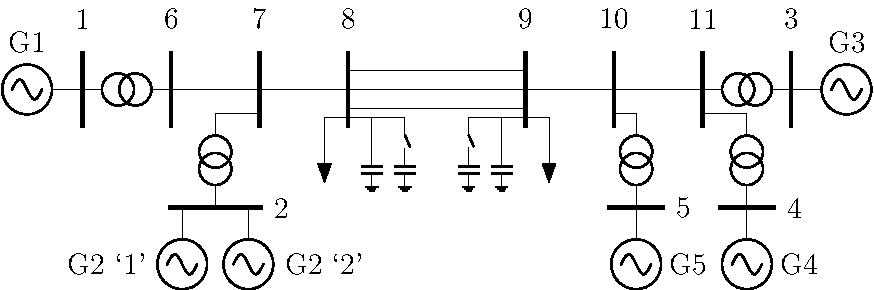
\includegraphics[width=\linewidth]{../../models/sixMachine/sixMachine}
\paragraph{Event and BA Description:} The simplest explanation is the code used to define the event, power plants, and BA.
\begin{Verbatim}
# Perturbances
mirror.sysPerturbances = [
    'load 9 : step P 5 75 rel', # Step Load P +75 MW relative at t=5
    ]

# Power Plants
# defined as a dictionary of lists {'name' : ['gen id : participation factor', ...], ...}
mirror.sysPowerPlants ={'pp1': ["gen 2 1: 0.75 : rampA", "gen 2 2 : 0.25: rampA"],
                        'pp2': ["gen 3 : 0.75: rampA", "gen 4 : 0.25: rampA"],
                        }

# Testing of Balancing Authority input
mirror.sysBA = {
    'BA1':{
        'Area':1,
        'B':" 1.0 : p", # MW/0.1 Hz
        'ActionTime': 5.00, # sends update signals as requred every x seconds
        'Type':'TLB', # Tie-Line Bias
        'Filtering': 'PI : 0.1 0.0001', # where 0.1 = Kp, and 0.0001 = a = Ki/Kp
        'CtrlGens': ['plant pp1 : .60 ',
                    'gen 1 : .40 : rampA']
        },
    'BA2':{
        'Area':2,
        'B':" 1.0 : p", # MW/0.1 Hz
        'ActionTime': 5.00,
        'Type':'TLB', # Tie-Line Bias
        'Filtering': 'PI : 0.1 0.0001',
        'CtrlGens': ['plant pp2 : 1.0 ']
        },
    }
\end{Verbatim}

\pagebreak

\paragraph{Results:} The filtered ACE (which is distributed to controlled generators Pref according to participation factor) is much smaller than the calculated ACE. This allows for governor action to take place with minimal interference. The 20 minute simulation took 76 seconds ($\approx$60\% of total time spent solving Power Flows).
\begin{figure}[h!]
		\centering
		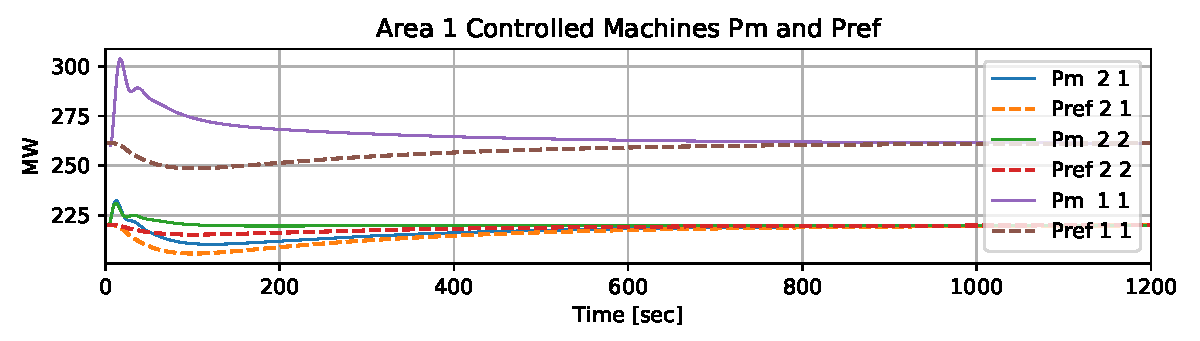
\includegraphics[width=\linewidth]{area1}\vspace{-1em}
		%\caption{Generator Electrical Power Output}
		%\label{ Pe}		 
\end{figure}\vspace{-1.5em}
\begin{figure}[h!]
		\centering
		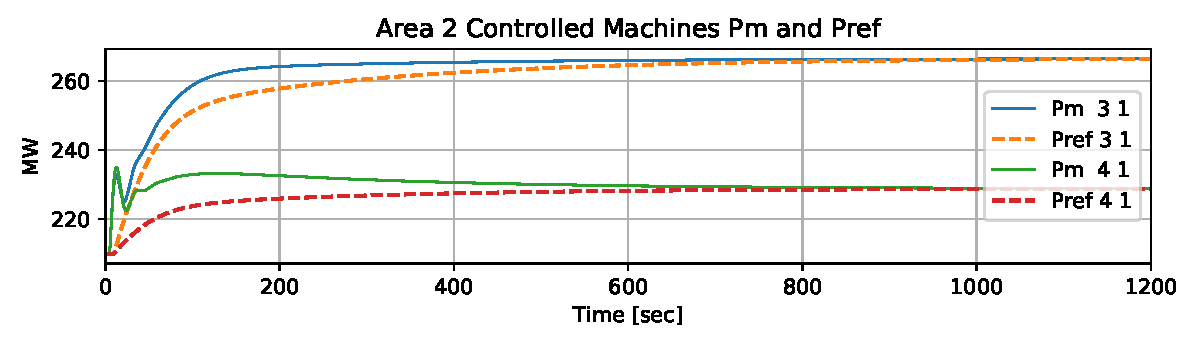
\includegraphics[width=\linewidth]{area2}\vspace{-1em}
		%\caption{Generator Mechanical Power Output (un-governed machines have no PSDS data)}
		%\label{ Pm}		 
\end{figure}\vspace{-1.5em}
\begin{figure}[h!]
		\centering
		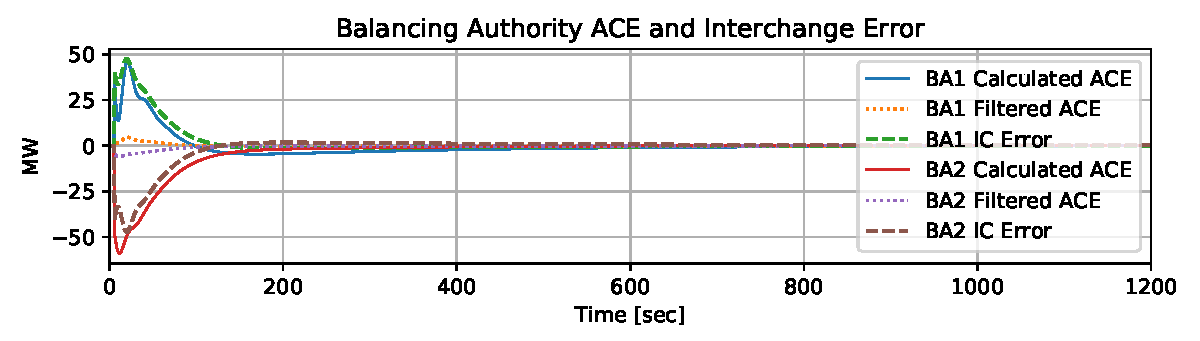
\includegraphics[width=\linewidth]{ace}\vspace{-1em}
		%\caption{Reactive Power Output}
		%\label{ Q}		 
\end{figure}\vspace{-1.5em}
\begin{figure}[h!]
		\centering
		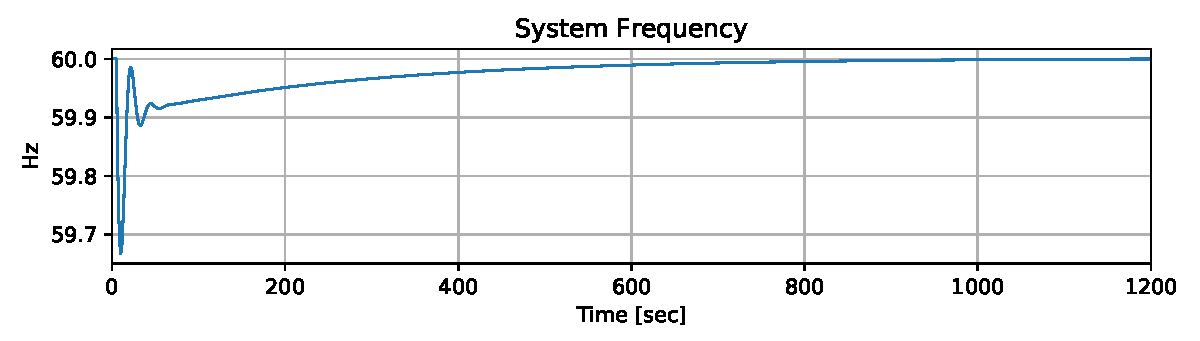
\includegraphics[width=\linewidth]{freq}\vspace{-1em}
		%\caption{Reactive Power Output}
		%\label{ Q}		 
\end{figure}\vspace{-1.5em}
\end{document}